% Created by tikzDevice version 0.12.6 on 2024-04-14 22:45:16
% !TEX encoding = UTF-8 Unicode
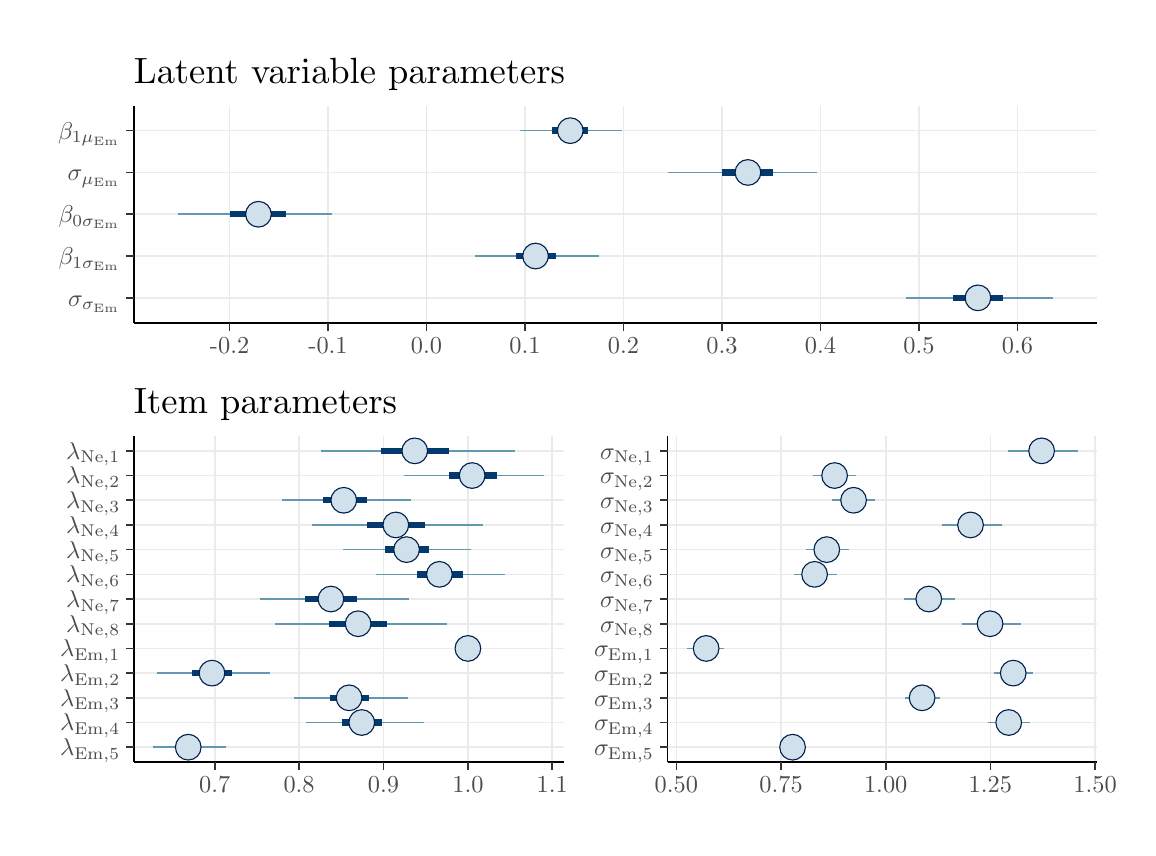
\begin{tikzpicture}[x=1pt,y=1pt]
\definecolor{fillColor}{RGB}{255,255,255}
\path[use as bounding box,fill=fillColor,fill opacity=0.00] (0,0) rectangle (397.48,289.08);
\begin{scope}
\path[clip] (  0.00,  0.00) rectangle (397.48,289.08);
\definecolor{drawColor}{RGB}{255,255,255}
\definecolor{fillColor}{RGB}{255,255,255}

\path[draw=drawColor,line width= 0.6pt,line join=round,line cap=round,fill=fillColor] (  0.00,  0.00) rectangle (397.48,289.08);
\end{scope}
\begin{scope}
\path[clip] (  5.50,164.17) rectangle (391.98,283.58);
\definecolor{drawColor}{RGB}{255,255,255}
\definecolor{fillColor}{RGB}{255,255,255}

\path[draw=drawColor,line width= 0.6pt,line join=round,line cap=round,fill=fillColor] (  5.50,164.17) rectangle (391.98,283.58);
\end{scope}
\begin{scope}
\path[clip] ( 38.38,182.39) rectangle (386.48,260.92);
\definecolor{fillColor}{RGB}{255,255,255}

\path[fill=fillColor] ( 38.38,182.39) rectangle (386.48,260.92);
\definecolor{drawColor}{gray}{0.92}

\path[draw=drawColor,line width= 0.6pt,line join=round] ( 38.38,191.45) --
	(386.48,191.45);

\path[draw=drawColor,line width= 0.6pt,line join=round] ( 38.38,206.56) --
	(386.48,206.56);

\path[draw=drawColor,line width= 0.6pt,line join=round] ( 38.38,221.66) --
	(386.48,221.66);

\path[draw=drawColor,line width= 0.6pt,line join=round] ( 38.38,236.76) --
	(386.48,236.76);

\path[draw=drawColor,line width= 0.6pt,line join=round] ( 38.38,251.86) --
	(386.48,251.86);

\path[draw=drawColor,line width= 0.6pt,line join=round] ( 72.96,182.39) --
	( 72.96,260.92);

\path[draw=drawColor,line width= 0.6pt,line join=round] (108.54,182.39) --
	(108.54,260.92);

\path[draw=drawColor,line width= 0.6pt,line join=round] (144.13,182.39) --
	(144.13,260.92);

\path[draw=drawColor,line width= 0.6pt,line join=round] (179.71,182.39) --
	(179.71,260.92);

\path[draw=drawColor,line width= 0.6pt,line join=round] (215.30,182.39) --
	(215.30,260.92);

\path[draw=drawColor,line width= 0.6pt,line join=round] (250.89,182.39) --
	(250.89,260.92);

\path[draw=drawColor,line width= 0.6pt,line join=round] (286.47,182.39) --
	(286.47,260.92);

\path[draw=drawColor,line width= 0.6pt,line join=round] (322.06,182.39) --
	(322.06,260.92);

\path[draw=drawColor,line width= 0.6pt,line join=round] (357.65,182.39) --
	(357.65,260.92);
\definecolor{drawColor}{gray}{0.90}

\path[draw=drawColor,line width= 0.6pt,line join=round] (144.13,182.39) -- (144.13,260.92);
\definecolor{drawColor}{RGB}{100,151,177}

\path[draw=drawColor,line width= 0.6pt,line join=round] (177.75,251.86) -- (214.76,251.86);

\path[draw=drawColor,line width= 0.6pt,line join=round] (231.32,236.76) -- (285.36,236.76);

\path[draw=drawColor,line width= 0.6pt,line join=round] ( 54.21,221.66) -- (109.99,221.66);

\path[draw=drawColor,line width= 0.6pt,line join=round] (161.59,206.56) -- (206.51,206.56);

\path[draw=drawColor,line width= 0.6pt,line join=round] (317.37,191.45) -- (370.66,191.45);
\definecolor{drawColor}{RGB}{3,57,108}

\path[draw=drawColor,line width= 2.3pt,line join=round] (189.38,251.86) -- (202.54,251.86);

\path[draw=drawColor,line width= 2.3pt,line join=round] (250.75,236.76) -- (269.26,236.76);

\path[draw=drawColor,line width= 2.3pt,line join=round] ( 73.09,221.66) -- ( 93.36,221.66);

\path[draw=drawColor,line width= 2.3pt,line join=round] (176.57,206.56) -- (190.94,206.56);

\path[draw=drawColor,line width= 2.3pt,line join=round] (334.34,191.45) -- (352.59,191.45);
\definecolor{drawColor}{RGB}{1,31,75}
\definecolor{fillColor}{RGB}{209,225,236}

\path[draw=drawColor,line width= 0.4pt,line join=round,line cap=round,fill=fillColor] (196.07,251.86) circle (  4.64);

\path[draw=drawColor,line width= 0.4pt,line join=round,line cap=round,fill=fillColor] (260.26,236.76) circle (  4.64);

\path[draw=drawColor,line width= 0.4pt,line join=round,line cap=round,fill=fillColor] ( 83.39,221.66) circle (  4.64);

\path[draw=drawColor,line width= 0.4pt,line join=round,line cap=round,fill=fillColor] (183.52,206.56) circle (  4.64);

\path[draw=drawColor,line width= 0.4pt,line join=round,line cap=round,fill=fillColor] (343.38,191.45) circle (  4.64);
\end{scope}
\begin{scope}
\path[clip] (  0.00,  0.00) rectangle (397.48,289.08);
\definecolor{drawColor}{RGB}{0,0,0}

\path[draw=drawColor,line width= 0.6pt,line join=round] ( 38.38,182.39) --
	( 38.38,260.92);
\end{scope}
\begin{scope}
\path[clip] (  0.00,  0.00) rectangle (397.48,289.08);
\definecolor{drawColor}{gray}{0.30}

\node[text=drawColor,anchor=base east,inner sep=0pt, outer sep=0pt, scale=  0.88] at ( 33.43,188.42) {$\sigma_{\sigma_\mathrm{Em}}$};

\node[text=drawColor,anchor=base east,inner sep=0pt, outer sep=0pt, scale=  0.88] at ( 33.43,203.53) {$\beta_{1 \sigma_\mathrm{Em}}$};

\node[text=drawColor,anchor=base east,inner sep=0pt, outer sep=0pt, scale=  0.88] at ( 33.43,218.63) {$\beta_{0 \sigma_\mathrm{Em}}$};

\node[text=drawColor,anchor=base east,inner sep=0pt, outer sep=0pt, scale=  0.88] at ( 33.43,233.73) {$\sigma_{\mu_\mathrm{Em}}$};

\node[text=drawColor,anchor=base east,inner sep=0pt, outer sep=0pt, scale=  0.88] at ( 33.43,248.83) {$\beta_{1 \mu_\mathrm{Em}}$};
\end{scope}
\begin{scope}
\path[clip] (  0.00,  0.00) rectangle (397.48,289.08);
\definecolor{drawColor}{gray}{0.20}

\path[draw=drawColor,line width= 0.6pt,line join=round] ( 35.63,191.45) --
	( 38.38,191.45);

\path[draw=drawColor,line width= 0.6pt,line join=round] ( 35.63,206.56) --
	( 38.38,206.56);

\path[draw=drawColor,line width= 0.6pt,line join=round] ( 35.63,221.66) --
	( 38.38,221.66);

\path[draw=drawColor,line width= 0.6pt,line join=round] ( 35.63,236.76) --
	( 38.38,236.76);

\path[draw=drawColor,line width= 0.6pt,line join=round] ( 35.63,251.86) --
	( 38.38,251.86);
\end{scope}
\begin{scope}
\path[clip] (  0.00,  0.00) rectangle (397.48,289.08);
\definecolor{drawColor}{RGB}{0,0,0}

\path[draw=drawColor,line width= 0.6pt,line join=round] ( 38.38,182.39) --
	(386.48,182.39);
\end{scope}
\begin{scope}
\path[clip] (  0.00,  0.00) rectangle (397.48,289.08);
\definecolor{drawColor}{gray}{0.20}

\path[draw=drawColor,line width= 0.6pt,line join=round] ( 72.96,179.64) --
	( 72.96,182.39);

\path[draw=drawColor,line width= 0.6pt,line join=round] (108.54,179.64) --
	(108.54,182.39);

\path[draw=drawColor,line width= 0.6pt,line join=round] (144.13,179.64) --
	(144.13,182.39);

\path[draw=drawColor,line width= 0.6pt,line join=round] (179.71,179.64) --
	(179.71,182.39);

\path[draw=drawColor,line width= 0.6pt,line join=round] (215.30,179.64) --
	(215.30,182.39);

\path[draw=drawColor,line width= 0.6pt,line join=round] (250.89,179.64) --
	(250.89,182.39);

\path[draw=drawColor,line width= 0.6pt,line join=round] (286.47,179.64) --
	(286.47,182.39);

\path[draw=drawColor,line width= 0.6pt,line join=round] (322.06,179.64) --
	(322.06,182.39);

\path[draw=drawColor,line width= 0.6pt,line join=round] (357.65,179.64) --
	(357.65,182.39);
\end{scope}
\begin{scope}
\path[clip] (  0.00,  0.00) rectangle (397.48,289.08);
\definecolor{drawColor}{gray}{0.30}

\node[text=drawColor,anchor=base,inner sep=0pt, outer sep=0pt, scale=  0.88] at ( 72.96,171.38) {-0.2};

\node[text=drawColor,anchor=base,inner sep=0pt, outer sep=0pt, scale=  0.88] at (108.54,171.38) {-0.1};

\node[text=drawColor,anchor=base,inner sep=0pt, outer sep=0pt, scale=  0.88] at (144.13,171.38) {0.0};

\node[text=drawColor,anchor=base,inner sep=0pt, outer sep=0pt, scale=  0.88] at (179.71,171.38) {0.1};

\node[text=drawColor,anchor=base,inner sep=0pt, outer sep=0pt, scale=  0.88] at (215.30,171.38) {0.2};

\node[text=drawColor,anchor=base,inner sep=0pt, outer sep=0pt, scale=  0.88] at (250.89,171.38) {0.3};

\node[text=drawColor,anchor=base,inner sep=0pt, outer sep=0pt, scale=  0.88] at (286.47,171.38) {0.4};

\node[text=drawColor,anchor=base,inner sep=0pt, outer sep=0pt, scale=  0.88] at (322.06,171.38) {0.5};

\node[text=drawColor,anchor=base,inner sep=0pt, outer sep=0pt, scale=  0.88] at (357.65,171.38) {0.6};
\end{scope}
\begin{scope}
\path[clip] (  0.00,  0.00) rectangle (397.48,289.08);
\definecolor{drawColor}{RGB}{0,0,0}

\node[text=drawColor,anchor=base west,inner sep=0pt, outer sep=0pt, scale=  1.32] at ( 38.38,268.99) {Latent variable parameters};
\end{scope}
\begin{scope}
\path[clip] (  5.50,  5.50) rectangle (199.17,164.17);
\definecolor{drawColor}{RGB}{255,255,255}
\definecolor{fillColor}{RGB}{255,255,255}

\path[draw=drawColor,line width= 0.6pt,line join=round,line cap=round,fill=fillColor] (  5.50,  5.50) rectangle (199.17,164.17);
\end{scope}
\begin{scope}
\path[clip] ( 38.38, 23.72) rectangle (193.67,141.52);
\definecolor{fillColor}{RGB}{255,255,255}

\path[fill=fillColor] ( 38.38, 23.72) rectangle (193.67,141.52);
\definecolor{drawColor}{gray}{0.92}

\path[draw=drawColor,line width= 0.6pt,line join=round] ( 38.38, 29.08) --
	(193.67, 29.08);

\path[draw=drawColor,line width= 0.6pt,line join=round] ( 38.38, 38.00) --
	(193.67, 38.00);

\path[draw=drawColor,line width= 0.6pt,line join=round] ( 38.38, 46.92) --
	(193.67, 46.92);

\path[draw=drawColor,line width= 0.6pt,line join=round] ( 38.38, 55.85) --
	(193.67, 55.85);

\path[draw=drawColor,line width= 0.6pt,line join=round] ( 38.38, 64.77) --
	(193.67, 64.77);

\path[draw=drawColor,line width= 0.6pt,line join=round] ( 38.38, 73.69) --
	(193.67, 73.69);

\path[draw=drawColor,line width= 0.6pt,line join=round] ( 38.38, 82.62) --
	(193.67, 82.62);

\path[draw=drawColor,line width= 0.6pt,line join=round] ( 38.38, 91.54) --
	(193.67, 91.54);

\path[draw=drawColor,line width= 0.6pt,line join=round] ( 38.38,100.47) --
	(193.67,100.47);

\path[draw=drawColor,line width= 0.6pt,line join=round] ( 38.38,109.39) --
	(193.67,109.39);

\path[draw=drawColor,line width= 0.6pt,line join=round] ( 38.38,118.31) --
	(193.67,118.31);

\path[draw=drawColor,line width= 0.6pt,line join=round] ( 38.38,127.24) --
	(193.67,127.24);

\path[draw=drawColor,line width= 0.6pt,line join=round] ( 38.38,136.16) --
	(193.67,136.16);

\path[draw=drawColor,line width= 0.6pt,line join=round] ( 67.57, 23.72) --
	( 67.57,141.52);

\path[draw=drawColor,line width= 0.6pt,line join=round] ( 98.07, 23.72) --
	( 98.07,141.52);

\path[draw=drawColor,line width= 0.6pt,line join=round] (128.57, 23.72) --
	(128.57,141.52);

\path[draw=drawColor,line width= 0.6pt,line join=round] (159.07, 23.72) --
	(159.07,141.52);

\path[draw=drawColor,line width= 0.6pt,line join=round] (189.57, 23.72) --
	(189.57,141.52);
\definecolor{drawColor}{RGB}{100,151,177}

\path[draw=drawColor,line width= 0.6pt,line join=round] (106.07,136.16) -- (176.16,136.16);

\path[draw=drawColor,line width= 0.6pt,line join=round] (136.05,127.24) -- (186.61,127.24);

\path[draw=drawColor,line width= 0.6pt,line join=round] ( 91.97,118.31) -- (138.45,118.31);

\path[draw=drawColor,line width= 0.6pt,line join=round] (102.81,109.39) -- (164.61,109.39);

\path[draw=drawColor,line width= 0.6pt,line join=round] (113.99,100.47) -- (160.13,100.47);

\path[draw=drawColor,line width= 0.6pt,line join=round] (125.89, 91.54) -- (172.30, 91.54);

\path[draw=drawColor,line width= 0.6pt,line join=round] ( 83.99, 82.62) -- (137.63, 82.62);

\path[draw=drawColor,line width= 0.6pt,line join=round] ( 89.31, 73.69) -- (151.58, 73.69);

\path[draw=drawColor,line width= 0.6pt,line join=round] (159.07, 64.77) -- (159.07, 64.77);

\path[draw=drawColor,line width= 0.6pt,line join=round] ( 46.69, 55.85) -- ( 87.64, 55.85);

\path[draw=drawColor,line width= 0.6pt,line join=round] ( 96.13, 46.92) -- (137.41, 46.92);

\path[draw=drawColor,line width= 0.6pt,line join=round] (100.57, 38.00) -- (143.03, 38.00);

\path[draw=drawColor,line width= 0.6pt,line join=round] ( 45.44, 29.08) -- ( 71.52, 29.08);
\definecolor{drawColor}{RGB}{3,57,108}

\path[draw=drawColor,line width= 2.3pt,line join=round] (127.65,136.16) -- (152.12,136.16);

\path[draw=drawColor,line width= 2.3pt,line join=round] (152.24,127.24) -- (169.53,127.24);

\path[draw=drawColor,line width= 2.3pt,line join=round] (106.69,118.31) -- (122.51,118.31);

\path[draw=drawColor,line width= 2.3pt,line join=round] (122.54,109.39) -- (143.62,109.39);

\path[draw=drawColor,line width= 2.3pt,line join=round] (128.97,100.47) -- (144.99,100.47);

\path[draw=drawColor,line width= 2.3pt,line join=round] (140.63, 91.54) -- (157.23, 91.54);

\path[draw=drawColor,line width= 2.3pt,line join=round] (100.32, 82.62) -- (118.85, 82.62);

\path[draw=drawColor,line width= 2.3pt,line join=round] (109.06, 73.69) -- (129.89, 73.69);

\path[draw=drawColor,line width= 2.3pt,line join=round] (159.07, 64.77) -- (159.07, 64.77);

\path[draw=drawColor,line width= 2.3pt,line join=round] ( 59.47, 55.85) -- ( 73.68, 55.85);

\path[draw=drawColor,line width= 2.3pt,line join=round] (109.15, 46.92) -- (123.17, 46.92);

\path[draw=drawColor,line width= 2.3pt,line join=round] (113.40, 38.00) -- (127.96, 38.00);

\path[draw=drawColor,line width= 2.3pt,line join=round] ( 53.69, 29.08) -- ( 62.71, 29.08);
\definecolor{drawColor}{RGB}{1,31,75}
\definecolor{fillColor}{RGB}{209,225,236}

\path[draw=drawColor,line width= 0.4pt,line join=round,line cap=round,fill=fillColor] (139.87,136.16) circle (  4.64);

\path[draw=drawColor,line width= 0.4pt,line join=round,line cap=round,fill=fillColor] (160.61,127.24) circle (  4.64);

\path[draw=drawColor,line width= 0.4pt,line join=round,line cap=round,fill=fillColor] (114.21,118.31) circle (  4.64);

\path[draw=drawColor,line width= 0.4pt,line join=round,line cap=round,fill=fillColor] (133.03,109.39) circle (  4.64);

\path[draw=drawColor,line width= 0.4pt,line join=round,line cap=round,fill=fillColor] (136.91,100.47) circle (  4.64);

\path[draw=drawColor,line width= 0.4pt,line join=round,line cap=round,fill=fillColor] (148.78, 91.54) circle (  4.64);

\path[draw=drawColor,line width= 0.4pt,line join=round,line cap=round,fill=fillColor] (109.58, 82.62) circle (  4.64);

\path[draw=drawColor,line width= 0.4pt,line join=round,line cap=round,fill=fillColor] (119.41, 73.69) circle (  4.64);

\path[draw=drawColor,line width= 0.4pt,line join=round,line cap=round,fill=fillColor] (159.07, 64.77) circle (  4.64);

\path[draw=drawColor,line width= 0.4pt,line join=round,line cap=round,fill=fillColor] ( 66.60, 55.85) circle (  4.64);

\path[draw=drawColor,line width= 0.4pt,line join=round,line cap=round,fill=fillColor] (116.15, 46.92) circle (  4.64);

\path[draw=drawColor,line width= 0.4pt,line join=round,line cap=round,fill=fillColor] (120.72, 38.00) circle (  4.64);

\path[draw=drawColor,line width= 0.4pt,line join=round,line cap=round,fill=fillColor] ( 58.02, 29.08) circle (  4.64);
\end{scope}
\begin{scope}
\path[clip] (  0.00,  0.00) rectangle (397.48,289.08);
\definecolor{drawColor}{RGB}{0,0,0}

\path[draw=drawColor,line width= 0.6pt,line join=round] ( 38.38, 23.72) --
	( 38.38,141.52);
\end{scope}
\begin{scope}
\path[clip] (  0.00,  0.00) rectangle (397.48,289.08);
\definecolor{drawColor}{gray}{0.30}

\node[text=drawColor,anchor=base east,inner sep=0pt, outer sep=0pt, scale=  0.88] at ( 33.43, 26.05) {$\lambda_{\mathrm{Em},5}$};

\node[text=drawColor,anchor=base east,inner sep=0pt, outer sep=0pt, scale=  0.88] at ( 33.43, 34.97) {$\lambda_{\mathrm{Em},4}$};

\node[text=drawColor,anchor=base east,inner sep=0pt, outer sep=0pt, scale=  0.88] at ( 33.43, 43.89) {$\lambda_{\mathrm{Em},3}$};

\node[text=drawColor,anchor=base east,inner sep=0pt, outer sep=0pt, scale=  0.88] at ( 33.43, 52.82) {$\lambda_{\mathrm{Em},2}$};

\node[text=drawColor,anchor=base east,inner sep=0pt, outer sep=0pt, scale=  0.88] at ( 33.43, 61.74) {$\lambda_{\mathrm{Em},1}$};

\node[text=drawColor,anchor=base east,inner sep=0pt, outer sep=0pt, scale=  0.88] at ( 33.43, 70.66) {$\lambda_{\mathrm{Ne},8}$};

\node[text=drawColor,anchor=base east,inner sep=0pt, outer sep=0pt, scale=  0.88] at ( 33.43, 79.59) {$\lambda_{\mathrm{Ne},7}$};

\node[text=drawColor,anchor=base east,inner sep=0pt, outer sep=0pt, scale=  0.88] at ( 33.43, 88.51) {$\lambda_{\mathrm{Ne},6}$};

\node[text=drawColor,anchor=base east,inner sep=0pt, outer sep=0pt, scale=  0.88] at ( 33.43, 97.44) {$\lambda_{\mathrm{Ne},5}$};

\node[text=drawColor,anchor=base east,inner sep=0pt, outer sep=0pt, scale=  0.88] at ( 33.43,106.36) {$\lambda_{\mathrm{Ne},4}$};

\node[text=drawColor,anchor=base east,inner sep=0pt, outer sep=0pt, scale=  0.88] at ( 33.43,115.28) {$\lambda_{\mathrm{Ne},3}$};

\node[text=drawColor,anchor=base east,inner sep=0pt, outer sep=0pt, scale=  0.88] at ( 33.43,124.21) {$\lambda_{\mathrm{Ne},2}$};

\node[text=drawColor,anchor=base east,inner sep=0pt, outer sep=0pt, scale=  0.88] at ( 33.43,133.13) {$\lambda_{\mathrm{Ne},1}$};
\end{scope}
\begin{scope}
\path[clip] (  0.00,  0.00) rectangle (397.48,289.08);
\definecolor{drawColor}{gray}{0.20}

\path[draw=drawColor,line width= 0.6pt,line join=round] ( 35.63, 29.08) --
	( 38.38, 29.08);

\path[draw=drawColor,line width= 0.6pt,line join=round] ( 35.63, 38.00) --
	( 38.38, 38.00);

\path[draw=drawColor,line width= 0.6pt,line join=round] ( 35.63, 46.92) --
	( 38.38, 46.92);

\path[draw=drawColor,line width= 0.6pt,line join=round] ( 35.63, 55.85) --
	( 38.38, 55.85);

\path[draw=drawColor,line width= 0.6pt,line join=round] ( 35.63, 64.77) --
	( 38.38, 64.77);

\path[draw=drawColor,line width= 0.6pt,line join=round] ( 35.63, 73.69) --
	( 38.38, 73.69);

\path[draw=drawColor,line width= 0.6pt,line join=round] ( 35.63, 82.62) --
	( 38.38, 82.62);

\path[draw=drawColor,line width= 0.6pt,line join=round] ( 35.63, 91.54) --
	( 38.38, 91.54);

\path[draw=drawColor,line width= 0.6pt,line join=round] ( 35.63,100.47) --
	( 38.38,100.47);

\path[draw=drawColor,line width= 0.6pt,line join=round] ( 35.63,109.39) --
	( 38.38,109.39);

\path[draw=drawColor,line width= 0.6pt,line join=round] ( 35.63,118.31) --
	( 38.38,118.31);

\path[draw=drawColor,line width= 0.6pt,line join=round] ( 35.63,127.24) --
	( 38.38,127.24);

\path[draw=drawColor,line width= 0.6pt,line join=round] ( 35.63,136.16) --
	( 38.38,136.16);
\end{scope}
\begin{scope}
\path[clip] (  0.00,  0.00) rectangle (397.48,289.08);
\definecolor{drawColor}{RGB}{0,0,0}

\path[draw=drawColor,line width= 0.6pt,line join=round] ( 38.38, 23.72) --
	(193.67, 23.72);
\end{scope}
\begin{scope}
\path[clip] (  0.00,  0.00) rectangle (397.48,289.08);
\definecolor{drawColor}{gray}{0.20}

\path[draw=drawColor,line width= 0.6pt,line join=round] ( 67.57, 20.97) --
	( 67.57, 23.72);

\path[draw=drawColor,line width= 0.6pt,line join=round] ( 98.07, 20.97) --
	( 98.07, 23.72);

\path[draw=drawColor,line width= 0.6pt,line join=round] (128.57, 20.97) --
	(128.57, 23.72);

\path[draw=drawColor,line width= 0.6pt,line join=round] (159.07, 20.97) --
	(159.07, 23.72);

\path[draw=drawColor,line width= 0.6pt,line join=round] (189.57, 20.97) --
	(189.57, 23.72);
\end{scope}
\begin{scope}
\path[clip] (  0.00,  0.00) rectangle (397.48,289.08);
\definecolor{drawColor}{gray}{0.30}

\node[text=drawColor,anchor=base,inner sep=0pt, outer sep=0pt, scale=  0.88] at ( 67.57, 12.71) {0.7};

\node[text=drawColor,anchor=base,inner sep=0pt, outer sep=0pt, scale=  0.88] at ( 98.07, 12.71) {0.8};

\node[text=drawColor,anchor=base,inner sep=0pt, outer sep=0pt, scale=  0.88] at (128.57, 12.71) {0.9};

\node[text=drawColor,anchor=base,inner sep=0pt, outer sep=0pt, scale=  0.88] at (159.07, 12.71) {1.0};

\node[text=drawColor,anchor=base,inner sep=0pt, outer sep=0pt, scale=  0.88] at (189.57, 12.71) {1.1};
\end{scope}
\begin{scope}
\path[clip] (  0.00,  0.00) rectangle (397.48,289.08);
\definecolor{drawColor}{RGB}{0,0,0}

\node[text=drawColor,anchor=base west,inner sep=0pt, outer sep=0pt, scale=  1.32] at ( 38.38,149.58) {Item parameters};
\end{scope}
\begin{scope}
\path[clip] (199.17,  5.50) rectangle (391.98,164.17);
\definecolor{drawColor}{RGB}{255,255,255}
\definecolor{fillColor}{RGB}{255,255,255}

\path[draw=drawColor,line width= 0.6pt,line join=round,line cap=round,fill=fillColor] (199.17,  5.50) rectangle (391.98,164.17);
\end{scope}
\begin{scope}
\path[clip] (231.20, 23.72) rectangle (386.48,141.52);
\definecolor{fillColor}{RGB}{255,255,255}

\path[fill=fillColor] (231.20, 23.72) rectangle (386.48,141.52);
\definecolor{drawColor}{gray}{0.92}

\path[draw=drawColor,line width= 0.6pt,line join=round] (231.20, 29.08) --
	(386.48, 29.08);

\path[draw=drawColor,line width= 0.6pt,line join=round] (231.20, 38.00) --
	(386.48, 38.00);

\path[draw=drawColor,line width= 0.6pt,line join=round] (231.20, 46.92) --
	(386.48, 46.92);

\path[draw=drawColor,line width= 0.6pt,line join=round] (231.20, 55.85) --
	(386.48, 55.85);

\path[draw=drawColor,line width= 0.6pt,line join=round] (231.20, 64.77) --
	(386.48, 64.77);

\path[draw=drawColor,line width= 0.6pt,line join=round] (231.20, 73.69) --
	(386.48, 73.69);

\path[draw=drawColor,line width= 0.6pt,line join=round] (231.20, 82.62) --
	(386.48, 82.62);

\path[draw=drawColor,line width= 0.6pt,line join=round] (231.20, 91.54) --
	(386.48, 91.54);

\path[draw=drawColor,line width= 0.6pt,line join=round] (231.20,100.47) --
	(386.48,100.47);

\path[draw=drawColor,line width= 0.6pt,line join=round] (231.20,109.39) --
	(386.48,109.39);

\path[draw=drawColor,line width= 0.6pt,line join=round] (231.20,118.31) --
	(386.48,118.31);

\path[draw=drawColor,line width= 0.6pt,line join=round] (231.20,127.24) --
	(386.48,127.24);

\path[draw=drawColor,line width= 0.6pt,line join=round] (231.20,136.16) --
	(386.48,136.16);

\path[draw=drawColor,line width= 0.6pt,line join=round] (234.40, 23.72) --
	(234.40,141.52);

\path[draw=drawColor,line width= 0.6pt,line join=round] (272.23, 23.72) --
	(272.23,141.52);

\path[draw=drawColor,line width= 0.6pt,line join=round] (310.05, 23.72) --
	(310.05,141.52);

\path[draw=drawColor,line width= 0.6pt,line join=round] (347.88, 23.72) --
	(347.88,141.52);

\path[draw=drawColor,line width= 0.6pt,line join=round] (385.71, 23.72) --
	(385.71,141.52);
\definecolor{drawColor}{RGB}{100,151,177}

\path[draw=drawColor,line width= 0.6pt,line join=round] (354.37,136.16) -- (379.43,136.16);

\path[draw=drawColor,line width= 0.6pt,line join=round] (283.65,127.24) -- (299.38,127.24);

\path[draw=drawColor,line width= 0.6pt,line join=round] (290.66,118.31) -- (306.24,118.31);

\path[draw=drawColor,line width= 0.6pt,line join=round] (330.55,109.39) -- (352.15,109.39);

\path[draw=drawColor,line width= 0.6pt,line join=round] (281.17,100.47) -- (296.83,100.47);

\path[draw=drawColor,line width= 0.6pt,line join=round] (276.89, 91.54) -- (292.30, 91.54);

\path[draw=drawColor,line width= 0.6pt,line join=round] (316.76, 82.62) -- (335.09, 82.62);

\path[draw=drawColor,line width= 0.6pt,line join=round] (337.72, 73.69) -- (358.93, 73.69);

\path[draw=drawColor,line width= 0.6pt,line join=round] (238.26, 64.77) -- (251.68, 64.77);

\path[draw=drawColor,line width= 0.6pt,line join=round] (349.22, 55.85) -- (363.43, 55.85);

\path[draw=drawColor,line width= 0.6pt,line join=round] (316.92, 46.92) -- (329.77, 46.92);

\path[draw=drawColor,line width= 0.6pt,line join=round] (346.83, 38.00) -- (362.02, 38.00);

\path[draw=drawColor,line width= 0.6pt,line join=round] (272.21, 29.08) -- (280.47, 29.08);
\definecolor{drawColor}{RGB}{3,57,108}

\path[draw=drawColor,line width= 2.3pt,line join=round] (361.96,136.16) -- (370.61,136.16);

\path[draw=drawColor,line width= 2.3pt,line join=round] (288.70,127.24) -- (294.35,127.24);

\path[draw=drawColor,line width= 2.3pt,line join=round] (295.61,118.31) -- (301.06,118.31);

\path[draw=drawColor,line width= 2.3pt,line join=round] (337.05,109.39) -- (344.41,109.39);

\path[draw=drawColor,line width= 2.3pt,line join=round] (286.26,100.47) -- (291.39,100.47);

\path[draw=drawColor,line width= 2.3pt,line join=round] (281.69, 91.54) -- (286.98, 91.54);

\path[draw=drawColor,line width= 2.3pt,line join=round] (322.56, 82.62) -- (328.86, 82.62);

\path[draw=drawColor,line width= 2.3pt,line join=round] (344.38, 73.69) -- (351.44, 73.69);

\path[draw=drawColor,line width= 2.3pt,line join=round] (242.85, 64.77) -- (247.50, 64.77);

\path[draw=drawColor,line width= 2.3pt,line join=round] (353.77, 55.85) -- (358.45, 55.85);

\path[draw=drawColor,line width= 2.3pt,line join=round] (321.04, 46.92) -- (325.46, 46.92);

\path[draw=drawColor,line width= 2.3pt,line join=round] (351.90, 38.00) -- (356.99, 38.00);

\path[draw=drawColor,line width= 2.3pt,line join=round] (274.94, 29.08) -- (277.82, 29.08);
\definecolor{drawColor}{RGB}{1,31,75}
\definecolor{fillColor}{RGB}{209,225,236}

\path[draw=drawColor,line width= 0.4pt,line join=round,line cap=round,fill=fillColor] (366.38,136.16) circle (  4.64);

\path[draw=drawColor,line width= 0.4pt,line join=round,line cap=round,fill=fillColor] (291.58,127.24) circle (  4.64);

\path[draw=drawColor,line width= 0.4pt,line join=round,line cap=round,fill=fillColor] (298.44,118.31) circle (  4.64);

\path[draw=drawColor,line width= 0.4pt,line join=round,line cap=round,fill=fillColor] (340.70,109.39) circle (  4.64);

\path[draw=drawColor,line width= 0.4pt,line join=round,line cap=round,fill=fillColor] (288.76,100.47) circle (  4.64);

\path[draw=drawColor,line width= 0.4pt,line join=round,line cap=round,fill=fillColor] (284.35, 91.54) circle (  4.64);

\path[draw=drawColor,line width= 0.4pt,line join=round,line cap=round,fill=fillColor] (325.62, 82.62) circle (  4.64);

\path[draw=drawColor,line width= 0.4pt,line join=round,line cap=round,fill=fillColor] (347.75, 73.69) circle (  4.64);

\path[draw=drawColor,line width= 0.4pt,line join=round,line cap=round,fill=fillColor] (245.16, 64.77) circle (  4.64);

\path[draw=drawColor,line width= 0.4pt,line join=round,line cap=round,fill=fillColor] (356.13, 55.85) circle (  4.64);

\path[draw=drawColor,line width= 0.4pt,line join=round,line cap=round,fill=fillColor] (323.20, 46.92) circle (  4.64);

\path[draw=drawColor,line width= 0.4pt,line join=round,line cap=round,fill=fillColor] (354.49, 38.00) circle (  4.64);

\path[draw=drawColor,line width= 0.4pt,line join=round,line cap=round,fill=fillColor] (276.39, 29.08) circle (  4.64);
\end{scope}
\begin{scope}
\path[clip] (  0.00,  0.00) rectangle (397.48,289.08);
\definecolor{drawColor}{RGB}{0,0,0}

\path[draw=drawColor,line width= 0.6pt,line join=round] (231.20, 23.72) --
	(231.20,141.52);
\end{scope}
\begin{scope}
\path[clip] (  0.00,  0.00) rectangle (397.48,289.08);
\definecolor{drawColor}{gray}{0.30}

\node[text=drawColor,anchor=base east,inner sep=0pt, outer sep=0pt, scale=  0.88] at (226.25, 26.05) {$\sigma_{\mathrm{Em},5}$};

\node[text=drawColor,anchor=base east,inner sep=0pt, outer sep=0pt, scale=  0.88] at (226.25, 34.97) {$\sigma_{\mathrm{Em},4}$};

\node[text=drawColor,anchor=base east,inner sep=0pt, outer sep=0pt, scale=  0.88] at (226.25, 43.89) {$\sigma_{\mathrm{Em},3}$};

\node[text=drawColor,anchor=base east,inner sep=0pt, outer sep=0pt, scale=  0.88] at (226.25, 52.82) {$\sigma_{\mathrm{Em},2}$};

\node[text=drawColor,anchor=base east,inner sep=0pt, outer sep=0pt, scale=  0.88] at (226.25, 61.74) {$\sigma_{\mathrm{Em},1}$};

\node[text=drawColor,anchor=base east,inner sep=0pt, outer sep=0pt, scale=  0.88] at (226.25, 70.66) {$\sigma_{\mathrm{Ne},8}$};

\node[text=drawColor,anchor=base east,inner sep=0pt, outer sep=0pt, scale=  0.88] at (226.25, 79.59) {$\sigma_{\mathrm{Ne},7}$};

\node[text=drawColor,anchor=base east,inner sep=0pt, outer sep=0pt, scale=  0.88] at (226.25, 88.51) {$\sigma_{\mathrm{Ne},6}$};

\node[text=drawColor,anchor=base east,inner sep=0pt, outer sep=0pt, scale=  0.88] at (226.25, 97.44) {$\sigma_{\mathrm{Ne},5}$};

\node[text=drawColor,anchor=base east,inner sep=0pt, outer sep=0pt, scale=  0.88] at (226.25,106.36) {$\sigma_{\mathrm{Ne},4}$};

\node[text=drawColor,anchor=base east,inner sep=0pt, outer sep=0pt, scale=  0.88] at (226.25,115.28) {$\sigma_{\mathrm{Ne},3}$};

\node[text=drawColor,anchor=base east,inner sep=0pt, outer sep=0pt, scale=  0.88] at (226.25,124.21) {$\sigma_{\mathrm{Ne},2}$};

\node[text=drawColor,anchor=base east,inner sep=0pt, outer sep=0pt, scale=  0.88] at (226.25,133.13) {$\sigma_{\mathrm{Ne},1}$};
\end{scope}
\begin{scope}
\path[clip] (  0.00,  0.00) rectangle (397.48,289.08);
\definecolor{drawColor}{gray}{0.20}

\path[draw=drawColor,line width= 0.6pt,line join=round] (228.45, 29.08) --
	(231.20, 29.08);

\path[draw=drawColor,line width= 0.6pt,line join=round] (228.45, 38.00) --
	(231.20, 38.00);

\path[draw=drawColor,line width= 0.6pt,line join=round] (228.45, 46.92) --
	(231.20, 46.92);

\path[draw=drawColor,line width= 0.6pt,line join=round] (228.45, 55.85) --
	(231.20, 55.85);

\path[draw=drawColor,line width= 0.6pt,line join=round] (228.45, 64.77) --
	(231.20, 64.77);

\path[draw=drawColor,line width= 0.6pt,line join=round] (228.45, 73.69) --
	(231.20, 73.69);

\path[draw=drawColor,line width= 0.6pt,line join=round] (228.45, 82.62) --
	(231.20, 82.62);

\path[draw=drawColor,line width= 0.6pt,line join=round] (228.45, 91.54) --
	(231.20, 91.54);

\path[draw=drawColor,line width= 0.6pt,line join=round] (228.45,100.47) --
	(231.20,100.47);

\path[draw=drawColor,line width= 0.6pt,line join=round] (228.45,109.39) --
	(231.20,109.39);

\path[draw=drawColor,line width= 0.6pt,line join=round] (228.45,118.31) --
	(231.20,118.31);

\path[draw=drawColor,line width= 0.6pt,line join=round] (228.45,127.24) --
	(231.20,127.24);

\path[draw=drawColor,line width= 0.6pt,line join=round] (228.45,136.16) --
	(231.20,136.16);
\end{scope}
\begin{scope}
\path[clip] (  0.00,  0.00) rectangle (397.48,289.08);
\definecolor{drawColor}{RGB}{0,0,0}

\path[draw=drawColor,line width= 0.6pt,line join=round] (231.20, 23.72) --
	(386.48, 23.72);
\end{scope}
\begin{scope}
\path[clip] (  0.00,  0.00) rectangle (397.48,289.08);
\definecolor{drawColor}{gray}{0.20}

\path[draw=drawColor,line width= 0.6pt,line join=round] (234.40, 20.97) --
	(234.40, 23.72);

\path[draw=drawColor,line width= 0.6pt,line join=round] (272.23, 20.97) --
	(272.23, 23.72);

\path[draw=drawColor,line width= 0.6pt,line join=round] (310.05, 20.97) --
	(310.05, 23.72);

\path[draw=drawColor,line width= 0.6pt,line join=round] (347.88, 20.97) --
	(347.88, 23.72);

\path[draw=drawColor,line width= 0.6pt,line join=round] (385.71, 20.97) --
	(385.71, 23.72);
\end{scope}
\begin{scope}
\path[clip] (  0.00,  0.00) rectangle (397.48,289.08);
\definecolor{drawColor}{gray}{0.30}

\node[text=drawColor,anchor=base,inner sep=0pt, outer sep=0pt, scale=  0.88] at (234.40, 12.71) {0.50};

\node[text=drawColor,anchor=base,inner sep=0pt, outer sep=0pt, scale=  0.88] at (272.23, 12.71) {0.75};

\node[text=drawColor,anchor=base,inner sep=0pt, outer sep=0pt, scale=  0.88] at (310.05, 12.71) {1.00};

\node[text=drawColor,anchor=base,inner sep=0pt, outer sep=0pt, scale=  0.88] at (347.88, 12.71) {1.25};

\node[text=drawColor,anchor=base,inner sep=0pt, outer sep=0pt, scale=  0.88] at (385.71, 12.71) {1.50};
\end{scope}
\end{tikzpicture}
